%% Lab Report for EEET2493_labreport_template.tex
%% V1.0
%% 2019/01/16
%% This is the template for a Lab report following an IEEE paper. Modified by Francisco Tovar after Michael Sheel original document.


%% This is a skeleton file demonstrating the use of IEEEtran.cls
%% (requires IEEEtran.cls version 1.8b or later) with an IEEE
%% journal paper.
%%
%% Support sites:
%% http://www.michaelshell.org/tex/ieeetran/
%% http://www.ctan.org/pkg/ieeetran
%% and
%% http://www.ieee.org/

%%*************************************************************************
%% Legal Notice:
%% This code is offered as-is without any warranty either expressed or
%% implied; without even the implied warranty of MERCHANTABILITY or
%% FITNESS FOR A PARTICULAR PURPOSE! 
%% User assumes all risk.
%% In no event shall the IEEE or any contributor to this code be liable for
%% any damages or losses, including, but not limited to, incidental,
%% consequential, or any other damages, resulting from the use or misuse
%% of any information contained here.
%%
%% All comments are the opinions of their respective authors and are not
%% necessarily endorsed by the IEEE.
%%
%% This work is distributed under the LaTeX Project Public License (LPPL)
%% ( http://www.latex-project.org/ ) version 1.3, and may be freely used,
%% distributed and modified. A copy of the LPPL, version 1.3, is included
%% in the base LaTeX documentation of all distributions of LaTeX released
%% 2003/12/01 or later.
%% Retain all contribution notices and credits.
%% ** Modified files should be clearly indicated as such, including  **
%% ** renaming them and changing author support contact information. **
%%*************************************************************************

\documentclass[journal]{IEEEtran}

% *** CITATION PACKAGES ***
\usepackage[style=ieee]{biblatex} 
\bibliography{example_bib.bib}    %your file created using JabRef

% *** MATH PACKAGES ***
\usepackage{amsmath}
\usepackage{comment}

\usepackage{tabularx} % en el preámbulo
\usepackage{caption}
\captionsetup{font=small, labelfont=bf, textfont=normalfont}

% *** PDF, URL AND HYPERLINK PACKAGES ***
\usepackage{url}
% correct bad hyphenation here
\hyphenation{op-tical net-works semi-conduc-tor}
\usepackage{graphicx}  %needed to include png, eps figures
\usepackage{float}  % used to fix location of images i.e.\begin{figure}[H]

\begin{document}


% paper title
\title{Rectificadores de media onda, onda completa y recortadores\\ \small{Práctica No. 2}}

% author names and affiliations
\author{
    \IEEEauthorblockN{Flores Cornejo Gustavo Mauricio, Muñoz Reyes Arturo Yabed, Morales Vásquez Miguel Ehecatl}\\
    \IEEEauthorblockA{\textit{Unidad Profesional Interdisciplinaria en Ingeniería y Tecnologías Avanzadas, IPN}}
}
        
% The report headers
\markboth{1MV12 Fundamentos de Electrónica. Práctica 2, Marzo 2026}%do not delete next lines
{Shell \MakeLowercase{\textit{et al.}}: Bare Demo of IEEEtran.cls for IEEE Journals}

% make the title area
\maketitle

% As a general rule, do not put math, special symbols or citations
% in the abstract or keywords.
\begin{abstract}
    This laboratory practice aims primarily to analyze the current–voltage (I–V) characteristic curves of the semiconductor diode in its forward and reverse bias regions. Two different devices were used—the 1N4001 rectifier and the 1N4148 fast-switching diode—to compare their operating parameters.

The study is divided into four phases: static verification using a multimeter, manual acquisition of I–V data, dynamic visualization through an oscilloscope in XY mode, and analysis of thermal behavior through simulation.

The results make it possible to validate the mathematical model given by the Shockley equation, demonstrating the nonlinear nature of the component and the critical influence of temperature on the threshold voltage and reverse saturation current.

\end{abstract}

\section{Introducción}
% Here we have the typical use of a "W" for an initial drop letter
% and "RITE" in caps to complete the first word.
% You must have at least 2 lines in the paragraph with the drop letter
% (should never be an issue)

\IEEEPARstart{E}l trabajo presente pretende reforzar las bases teóricas que rigen el comportamiento de un diodo, aplicarlas en práctica y entender los resultados físicos obtenidos. Para esto, se trabajará con dos diodos de silicio, el 1N4001 y el 1N4148.
La importancia de esta práctica es entender cómo y de qué manera pueden ser implementados estos componentes en circuitos electrónicos, además de comprender cómo los parámetros de éstos cambian al alterar algunos factores como lo es la temperatura.
Durante el desarrollo del trabajo presente se analizará y comprenderá la diferencia al analizar al diodo como un elemento ideal y como un elemento real que alteran los resultados finales.
Al término de esta práctica se espera que sea evidente el comportamiento de un diodo, tanto en su región de polarización directa como la de la polarización inversa, además de poder analizar circuitos donde se implementen este tipo de componentes para poder 
desglozar el funcionamiento y alteraciones en la salida.

\section{Objetivos}
La presente práctica tiene como objetivo conocer las curvas de I-V del diodo en sus regiones directa e inversa, y comprobar las curvas del diodo como semiconductor.
\section{Marco teórico}
\subsection{Diodo.} 
El diodo es un dispositivo semiconductor de dos terminales que permite el flujo de corriente en una sola dirección, actuando esencialmente como un interruptor unidireccional. Los diodos tienen una polaridad determinada por su ánodo (terminal positiva) y su cátodo (terminal negativa).

Si observamos el diagrama esquemático del diodo, la flecha apunta en sentido contrario al flujo real de electrones, esto debido a que es más fácil interpretar el flujo de la corriente adoptando el sentido convencional, facilitando así los cálculos y deducciones.

\subsection{Polarización.}
Decimos que un diodo tiene polarización directa cuando permite el paso de la corriente, lo cual ocurre cuando hay un potencial mayor en el ánodo que en el cátodo (superando el voltaje de umbral). Contrariamente, se tiene una polarización inversa cuando actúa como un aislante, impidiendo el paso de la corriente y actuando como un interruptor abierto. 

\subsection{Polarización Inversa.}
Cuando el ánodo del diodo se conecta al potencial negativo de la fuente y el cátodo al positivo, el dispositivo se encuentra en \textbf{polarización inversa}. En esta condición, el campo eléctrico externo se suma al campo interno de la unión p-n, provocando que la región de agotamiento se ensanche. Como consecuencia, aumenta la barrera de potencial y se dificulta aún más el paso de portadores mayoritarios.

En un diodo ideal, la corriente en polarización inversa sería exactamente cero. Sin embargo, en un diodo real siempre existe una pequeña corriente denominada \textbf{corriente de saturación inversa} o \textbf{corriente de fuga} ($I_S$). Esta corriente se debe principalmente al movimiento de portadores minoritarios que atraviesan la unión debido a la energía térmica del material semiconductor.

La ecuación completa del diodo describe este comportamiento:

\begin{equation} I_D = I_S \left( e^{\frac{V_D}{n V_T}} - 1 \right) \end{equation}
Esta ecuación es llamada la Ecuación de Shockley y ayuda para describir de manera matemática el comportamiento del dido.
Donde:
\begin{itemize}
    \item $I_S$ (Corriente de saturación inversa): Es la corriente mínima que fluye cuando el diodo está polarizado en inversa.
    
    \item $V_T$ (Voltaje térmico): Es el parámetro clave que vincula la energía térmica con el comportamiento eléctrico. Se calcula como:
    
    \[
        V_T = \frac{kT}{q}
    \]
\end{itemize}
Su funcionamiento del diodo es altamente sensible a los cambios térmicos debido a la naturaleza de los materiales semiconductores. 
Por ejemplo, el voltaje térmico actúa como un factor de escala dentro del exponente, lo que significa que define la pendiente de la 
curva una vez superado el voltaje de umbral. De igual forma la corriente de fuga es extremadamente sensible al calor; un aumento de 
temperatura incrementa drásticamente esta corriente de fuga.

Para valores negativos grandes de $V_D$, el término exponencial tiende a cero y la corriente se aproxima a:

\[
I \approx -I_S
\]

\subsection{Voltaje de umbral.}
Esla tensión a partir de la cual la corriente empieza a incrementarse rápidamente. Típicamente es de 0.7V para los diodos de silicio y 0.3 para los diodos de germanio.

\subsection{Inspección de un diodo.}
Para saber si un diodo es funcional configurado en la función de prueba de diodos. En este modo, el instrumento produce un pequeño voltaje entre sus terminales, al aplicar este potencial en polarización directa se obtiene una caída de tensión entre 0.5 a 0.8 V. También es factible comprobar la resistencia que tiene el diodo, un buen diodo polarizado directamente debería dar una lectura entre 10 a 1,000 ohm (dependiendo de la escala). Por el contrario, en polarización inversa el diodo debe registrar una lectura de circuito abierto (indicado como “OL”), esto indica que no deja pasar corriente en ese sentido.


\subsection{Dopaje de un diodo y diferencias.}
La esencia del diodo reside en la unión de dos tipos de estructuras cristalinas, dopadas de distinta manera, es decir, se le han añadido de forma controlada
 pequeñas cantidades de impurezas. El material tipo P cuenta con una abundancia de "huecos" (ausencia de electrones), mientras que el material tipo N posee un
  exceso de electrones libres Dependiendo de su construcción física y dopaje, se obtendrán distintos comportamientos y capacidades. Por ejemplo, al comparar la 
  familia 1N4000 (diodos rectificadores) con diodos de conmutación rápida como el 1N4148, se obtienen las siguientes diferencias.

\subsection{Comportamiento capacitivo del diodo}

Además de su comportamiento como rectificador, el diodo presenta capacitancia interna debido a la estructura de la unión p-n. Esto implica que, especialmente en señales de corriente alterna y altas frecuencias, el diodo puede comportarse como un capacitor dependiente del voltaje aplicado.

\[
C_j \propto \frac{1}{\sqrt{V_R}}
\]

Esta capacitancia es relevante en:

\begin{itemize}
    \item Circuitos de alta frecuencia.
    \item Aplicaciones de radiofrecuencia (RF).
    \item Velocidad de conmutación.
\end{itemize}

El 1N4148 posee menor capacitancia de unión que el 1N4001, lo que contribuye a su mayor rapidez de respuesta.


\begin{table}[H]
\centering
\begin{tabularx}{\columnwidth}{|c|X|X|X|X|}
\hline
\textbf{Parámetro} & \textbf{1N4001 (Rectificador)} & \textbf{1N4148 (Señal/Rápido)} \\ \hline
Voltaje de activación (VD) & $\approx$0.7V (Máx 1.1V a 1A) & $\approx$0.6V a 0.7V (Máx 1V a 10mA) \\ \hline
Voltaje Pico Inverso (VRRM) & 50V & 100V \\ \hline
Corriente Máx. Directa (IF) & 1.0A & 150mA a 300mA \\ \hline
Corriente Pico Inverso (IR) & 5$\mu$A (muy baja) & 25nA (extremadamente baja) \\ \hline
Frecuencia / Velocidad & Baja (60Hz) & Muy Alta (trr < 4ns) \\ \hline
Potencia de operación (PD) & 3W (típico con disipación) & 500mW \\ \hline
Temperatura de operación & -65$^\circ$C a +175$^\circ$C & -65$^\circ$C a +200$^\circ$C \\ \hline
\end{tabularx}
\caption{Comparación de especificaciones entre un diodo 1N4001 y un 1N4148.}
\label{tablaComparacionDiodos}
\end{table}

\begin{table}[H]
\centering
\begin{tabularx}{\columnwidth}{|c|X|X|}
\hline
\textbf{Tipo de Diodo} & \textbf{Funcionamiento Clave} & \textbf{Aplicaciones Comunes} \\ \hline
Rectificador & Pasa grandes corrientes en una sola dirección. & Fuentes de alimentación, cargadores. \\ \hline
De Señal & Conmutación extremadamente rápida. & Procesamiento de datos, lógica digital. \\ \hline
Zener & Conduce en inversa a un voltaje específico y estable. & Reguladores de voltaje, protección de circuitos. \\ \hline
Schottky & Caída de tensión muy baja (0.2V) y alta velocidad. & Fuentes conmutadas, paneles solares. \\ \hline
LED & Emite fotones cuando circula corriente. & Indicadores, iluminación, pantallas. \\ \hline
Fotodiodo & Genera corriente al recibir luz. & Sensores de luz, receptores de control remoto. \\ \hline
Varactor & Actúa como un capacitor variable mediante voltaje. & Sintonizadores de radio y TV (RF). \\ \hline
\end{tabularx}
\caption{Clasificación de diodos en base a sus aplicaciones.}
\label{tablaClasificacionDiodos}
\end{table}


\section{Materiales}

\begin{figure}[H]%[!ht]
\begin {center}

\includegraphics[width=0.45\textwidth]{IMAGENES/PRUEBA.jpg}
\caption{Circuito con diodo 1N4001.}
\label{fig:circuito_base1}
\end {center}
\end{figure}

Para el circuito mostrado en la "Figura~\ref{fig:circuito_base1}”, emplearemos:
\begin{itemize}
    \item 1 Diodo 1N4001
    \item 1 Diodo 1N4148
    \item 1 Resistencia de 220 $\Omega$
    \item Protoboard
    \item Cable para protoboard
\end{itemize}

La fuente V1 mostrada en la "Figura~\ref{fig:circuito_base1}” es una fuente variable que nos ayudará a analizar el 
comportamiento del diodo a diferentes valores de voltaje de entrada. Cabe aclarar que los diodos con los que se trabajará están 
hechos a base de silicio.

\section{Análisis y Resultados}
\subsection{Comprtamiento del transformador}
En esta sección se presentan y analizan las mediciones fundamentales del transformador reductor. Iniciamos con la 
identificación de los devanados (primario y secundario) y su derivación central a partir de la medición de sus resistencias. 
Posteriormente, con el equipo energizado, se documentan los voltajes RMS para determinar su relación de transformación. 
Finalmente, se verifica el desfasamiento de 180 grados entre las terminales, comprobando la suma de potenciales de extremo a extremo.

Para la caracterización inicial sin energizar, se midió la resistencia de las terminales para identificar los devanados. 
El devanado primario registró una resistencia de 112.4 $\Omega $. Por su parte, el devanado secundario presentó una resistencia total 
de 1.8 $\Omega $ medido de extremo a extremo. Al medir desde los extremos hacia la derivación central, se obtuvo una lectura de 0.9 $\Omega $, 
lo cual representa exactamente la mitad de la medición total y confirma la simetría del componente.

Posteriormente, al conectar el transformador a la toma de corriente de 120 $Vrms$ , se registró un voltaje de salida en el primario de $V_p = 120 Vrms$ (igual al de la fuente)
y en el secundario presentó un voltaje de $V_s = 13.21 Vrms$ de extremo a extremo. Con los datos obtenidos, podemos determinar el valor de la relacion de transformación (n)
del componente, para esto se calculó la proporción entre el voltaje suministrado al devanado primario ($Vp$) y el voltaje medido en el devanado secundario ($V_s$). Obtenemos:

\[
        n = \frac{V_p}{V_s} = \frac{120}{13.21} = {9.08}
\]

Con esto podemos observar la relación de reducción, es decir, el cálculo arroja una relación de transformación de aproximadamente 9:1. Lo cual indica físicamente que por cada 9 espiras 
en el devanado primario, existe 1 espira en el secundario, confirmando la naturaleza reductora del transformador utilizado.

Al utilizar la derivación central del secundario como punto de referencia común (tierra) para el osciloscopio, se midieron simultáneamente los voltajes de las dos terminales restantes. 
Se pudo comprobar gráficamente un desfasamiento exacto de 180 grados  entre ambas señales como se muestra en la Figura \ref{fig:desfasamiento}.

\begin{figure}[H]%[!ht]
\begin {center}
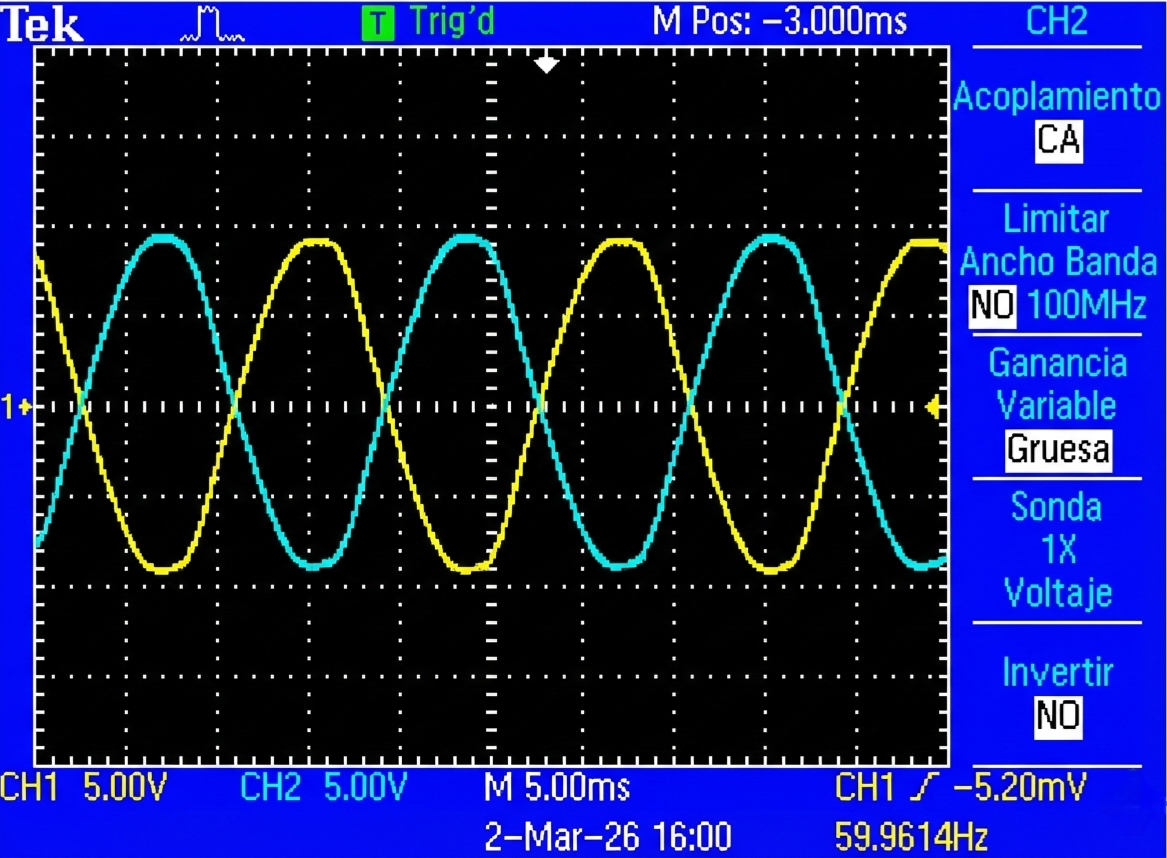
\includegraphics[width=0.45\textwidth]{IMAGENES/TRANSFORMADOR.png}
\caption{Desfasamiento de 180 grados en el transformador.}
\label{fig:desfasamiento}
\end {center}
\end{figure}

Este desfasamiento ocurre debido a la polaridad relativa inducida en la bobina. Según la Ley de Faraday, el flujo magnético alterno induce una diferencia de potencial a lo largo de 
todo el devanado secundario. Al "anclar" el centro físico de la bobina a 0V, el voltaje total se divide en dos mitades. En el instante en que la terminal superior es empujada hacia un 
potencial positivo máximo, la terminal inferior es forzada hacia un potencial negativo máximo de la misma magnitud para mantener la diferencia de potencial total. El resultado son dos 
señales senoidales que son el "espejo" la una de la otra.

Para corroborar la relación entre las señales, se procedió a medir con el osciloscopio la señal de extremo a extremo del secundario, omitiendo la derivación central.Cálculos teóricos: 
Por Ley de Voltajes de Kirchhoff, el voltaje total ($V_{total}$) es la diferencia de potencial entre la terminal superior ($V_A$) y la terminal inferior ($V_B$). Como se demostró en el inciso anterior 
que están desfasadas 180°, se cumple que $V_B(t) = -V_A(t)$. Por lo tanto, la sumatoria es:

\[
        V_{total} = V_A - V_B = V_A - (-V_A) = 2V_A
\]

Como se observó en la medición anterior, el voltaje pico en ambos canales respecto a la derivación central es de aproximadamente 9.3 V. Por consiguiente, por principio de suma de potenciales, la medición 
de extremo a extremo en el devanado secundario debe reflejar una amplitud equivalente al doble, alcanzando un valor pico cercano a los 18.6 V. Esta relación teórica se verifica de manera experimental en 
la Figura \ref{fig:comprobacion}

\begin{figure}[H]%[!ht]
\begin {center}
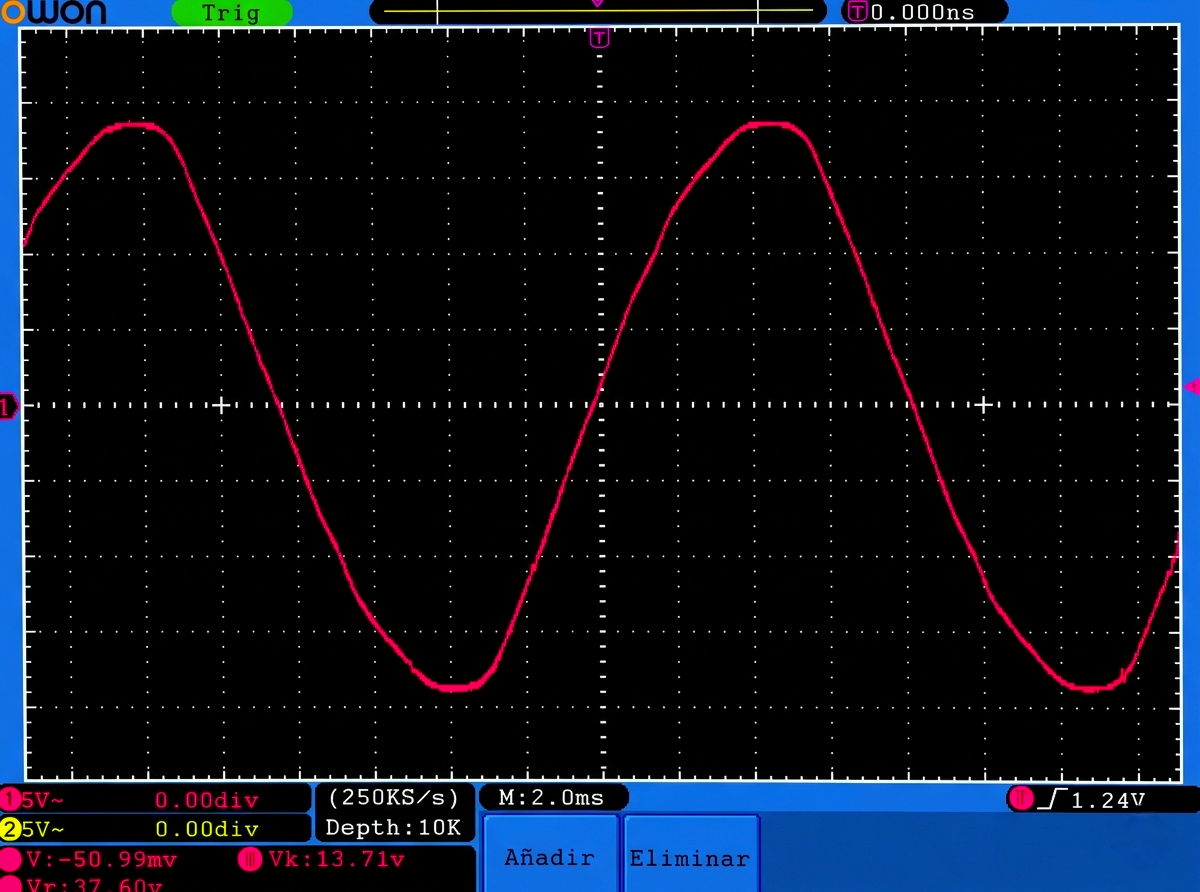
\includegraphics[width=0.45\textwidth]{IMAGENES/Comprobacion.png}
\caption{Medicion de extremo a extremo en el transformador.}
\label{fig:comprobacion}
\end {center}
\end{figure}

Al analizar la gráfica obtenida en el osciloscopio, la amplitud de la señal senoidal es exactamente el doble de la amplitud que se visualizó al medir solo una mitad contra la derivación central. 
Esto valida de forma práctica el principio de superposición y la naturaleza del desfasamiento de 180 grados inducido magnéticamente.

\subsection{Análisis del comportamiento del circuito 1}
En esta sección se evalúa el comportamiento de los diodos rectificadores utilizando la configuración de la Figura 1. Se determinaron los valores teóricos y prácticos del voltaje en la resistencia 
de carga ($R_1$), así como el voltaje de pico inverso (PIV) que soportan los semiconductores en estado de no conducción.

Para calcular el valtaje de la resistencia $R_1$, tomamos en cuenta los datos de las mediciones previas del transformador, en el cual se determinó que el voltaje eficaz total es de 13.21 Vrms (de extremo a extremo). 
Al utilizar la derivación central como referencia común, el voltaje eficaz para cada mitad del secundario es de 6.605 $V_{rms}$. El voltaje pico ($V_p$) proporcionado por cada canal hacia los diodos se calcula como:

\[
        V_p = 6.605 \cdot \sqrt{2}  = 9.34V
\]

Considerando el modelo práctico del diodo de silicio, el cual presenta una caída de tensión de aproximadamente 0.7V en polarización directa, el voltaje pico teórico esperado en la resistencia de carga ($V_{R1}$) es:

\[
    V_{R1} = 9.34 \text{ V} - 0.7 \text{ V} = 8.64 \text{ V}
\]

Al realizar la medición del voltaje $V_{R1}$ utilizando el osciloscopio, se obtuvieron los resultados de la forma de onda que se muestran en la Figura \ref{fig:voltajeResistencia}.

\begin{figure}[H]%[!ht]
\begin {center}
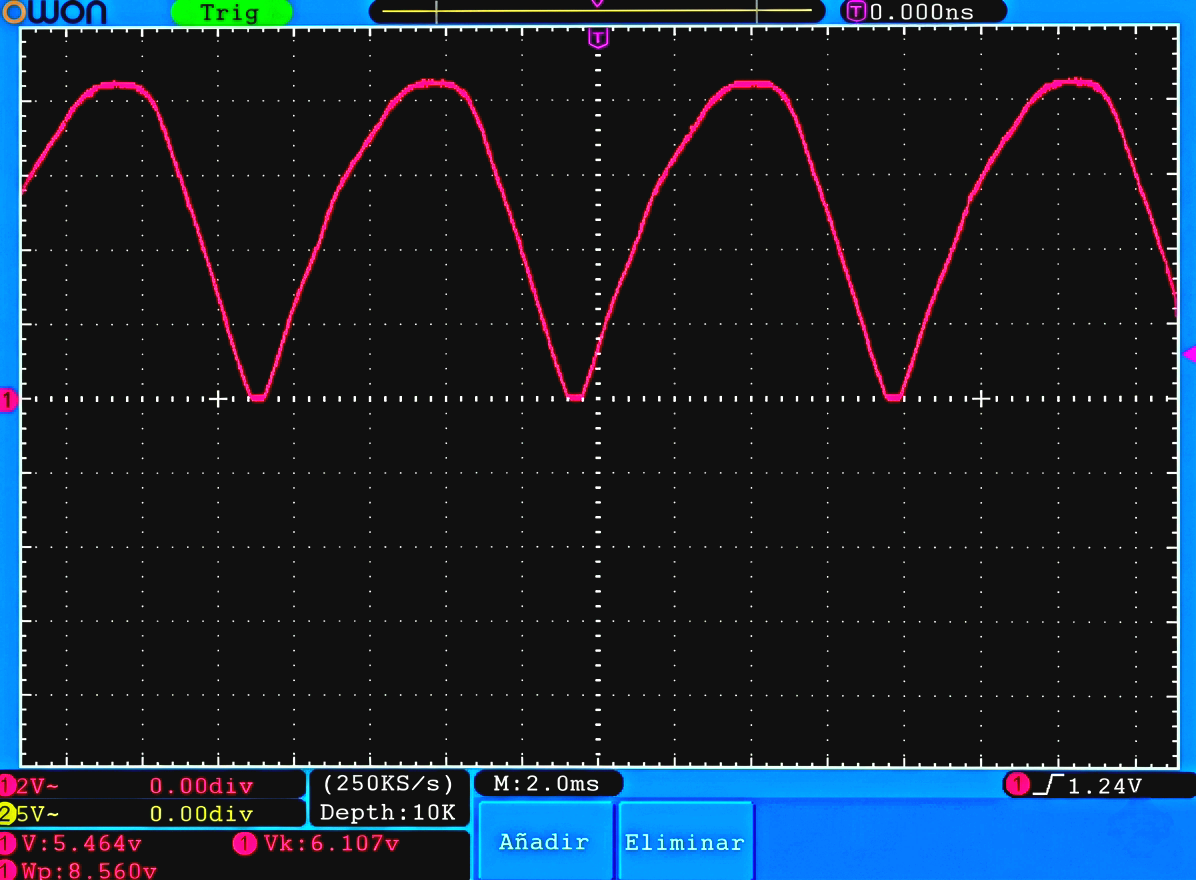
\includegraphics[width=0.45\textwidth]{IMAGENES/VoltajeResistencia.png}
\caption{Voltaje en la resistencia $R_1$}
\label{fig:voltajeResistencia}
\end {center}
\end{figure}

Para validar experimentalmente el análisis matemático, se efectuaron mediciones adicionales empleando un multímetro. A continuación, en la Tabla \ref{tablaComparativa}, se presenta una comparativa que contrasta 
los valores teóricos calculados para el voltaje en la resistencia de carga $R_1$ con las mediciones experimentales obtenidas tanto en el osciloscopio como con el multímetro.

\begin{table}[H]
\centering
\begin{tabularx}{\columnwidth}{|c|X|X|X|}
\hline
\textbf{Datos obtenidos} & \textbf{$V_prom$ (V)} & \textbf{$V_{rms}$ (V)} & \textbf{$V_{pp}$ (V)}\\ \hline
Multímetro & 5.17 & 5.89  & 8.03\\ \hline
Cálculos & 5.50 & 6.10  & 8.64\\ \hline
Osciloscopio & 5.464 & 6.107 & 8.560\\ \hline
\end{tabularx}
\caption{Comparacion de voltajes calculados y medidos de $R_1$.}
\label{tablaComparativa}
\end{table}

Ahora vamos a comprobar el voltaje inverso de ambos diodos dentro del circuito. Para esto utilizamos la ley de kirchoff (dos mallas), para realizar el análisis para D1 tenemos que hacerlo desde el semiciclo negativo, ya 
que es donde este no conduce. En este estado, el diodo $D_1$ entra en estado de bloqueo ($I_{D1}=0$), mientras que el diodo $D_2$ conduce, asumiendo una caída de tensión típica de $V_{D2} = 0.7 V$. Con esto establecemos la
siguiente relación:

\[
    -V_1 - V_2 - V_{D1} + V_{D2} = 0
\]
Donde $V_1$ es el voltaje del primer inductor y $V_2$ es el del segundo inductor.

Sustituyendo los valores ya anteriormente calculados ($V_1 = V_1 = 9.34 V_{rms}$). Obtenemos

\[
    V_{D1} = -2(9.34)+0.5 = -17.98 V
\]

Por lo tanto, el voltaje inverso teórico que soporta el semiconductor en estado de no conducción es de aproximadamente $-17.98 \text{ V}$. (La de ambos diodos)

Para demostrar experimentalmente este comportamiento en el osciloscopio, se configuró la función matemática (MATH) para calcular la diferencia de potencial, estableciendo el Canal A en el cátodo y el Canal B en el ánodo 
del diodo (A-B). Los resultados de esta configuración se observan en la Figura \ref{fig:voltajeInverso}.

\begin{figure}[H]%[!ht]
\begin{center}
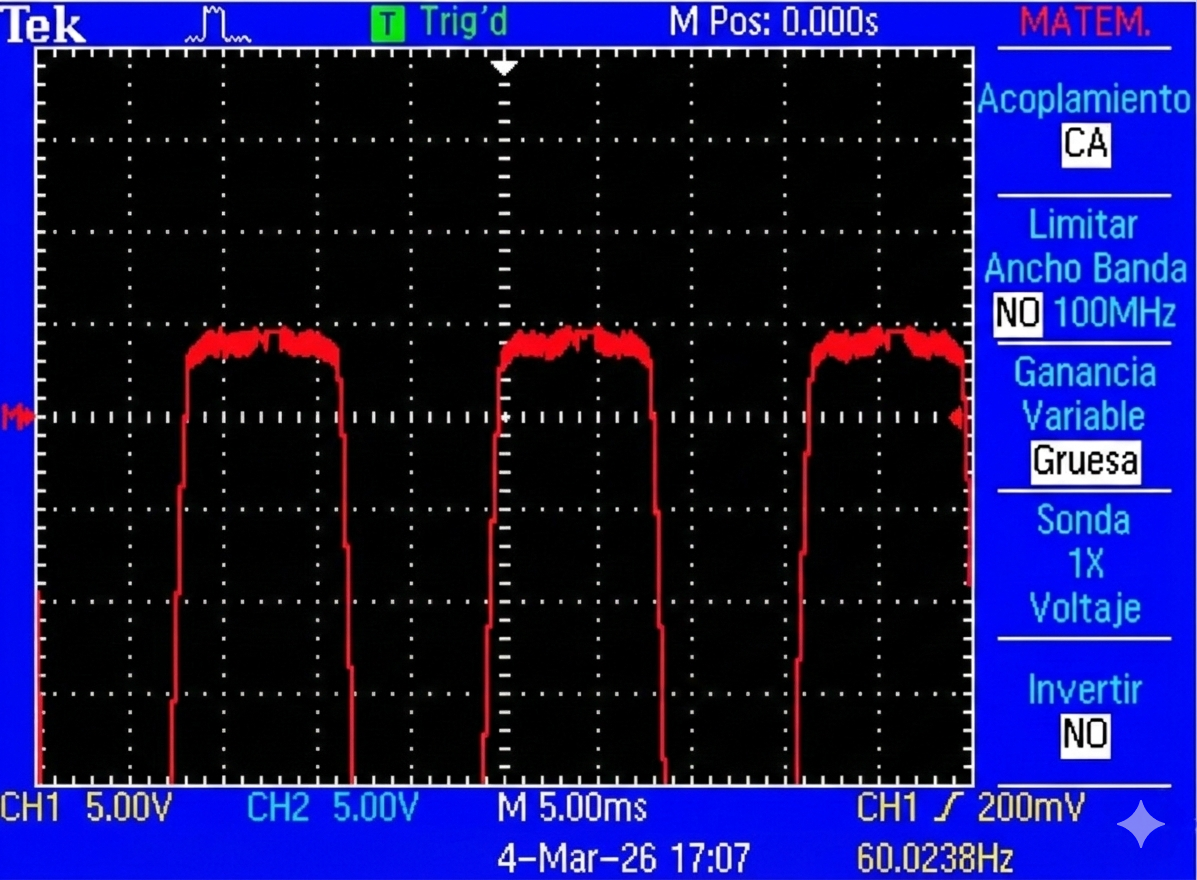
\includegraphics[width=0.45\textwidth]{IMAGENES/Voltaje_D1.png} 
\caption{Medición diferencial del voltaje en el diodo $D_1$.}
\label{fig:voltajeInverso}
\end{center}
\end{figure}

A continuación, se presenta una tabla comparativa entre el valor teórico calculado y la medición extraída del osciloscopio.

\begin{table}[H]
\centering
\begin{tabularx}{\columnwidth}{|c|X|}
\hline
\textbf{Método de obtención} & \textbf{Voltaje Inverso (V)} \\ \hline
Cálculo Teórico & -17.98 \\ \hline
Osciloscopio (MATH) & -18.20 \\ \hline
\end{tabularx}
\caption{Comparación del voltaje inverso en el diodo $D_1$.}
\label{tab:comparacion_PIV}
\end{table}

En la gráfica diferencial obtenida (trazo rojo), se comprueba de manera visual y cuantitativa el comportamiento bidireccional del componente. Durante el semiciclo positivo, el diodo conduce y la diferencia de potencial 
es mínima (cercana a los 0.7 V de la barrera de potencial). Sin embargo, durante el semiciclo negativo, la señal desciende hacia la región negativa. La diferencia observada entre el valor teórico ($-17.98 \text{ V}$) y el experimental 
se atribuye a la tolerancia de los componentes, la resolución del muestreo digital del osciloscopio al usar la función matemática a esa escala, y a las ligeras caídas de tensión en las líneas de conexión.

Para complementar la caracterización del semiconductor, se procedió a determinar la corriente que atraviesa el diodo $D_1$ durante su estado de conducción (semiciclo positivo).
La corriente pico ($I_{D1}$) en el circuito se define por la Ley de Ohm, considerando el voltaje pico en la carga ($V_R1$) y el valor de la resistencia $R_1$ ($220 \Omega$ ). Tomando el voltaje pico real previamente calculado (8.64 V), se tiene:
\[
    I_{D1 } = \frac{V_{R1}}{220} = \frac{8.64}{220} = 0.0392 A
\]

Dado que cada diodo en esta configuración conduce únicamente durante medio ciclo de la señal alterna, la corriente promedio ($I_{prom}$) y la corriente eficaz ($I_{rms}$) que soporta individualmente el componente se calculan con las fórmulas 
de rectificación de media onda:

\[
    I_{prom} = \frac{I_{D1}}{\pi} = \frac{0.0392}{\pi} = 12.47 mA
\]

\[
    I_{rms} = \frac{I_{D1}}{2} = \frac{0.0392}{2} = 19.60 mA
\]

Debido a que el osciloscopio mide diferencias de potencial y no corriente directa, se implementó una técnica de medición indirecta. Se insertó una resistencia de prueba de $1 \ \Omega$ en serie con el diodo $D_1$ . Por la Ley de Ohm ($V = I \cdot R$), 
al ser la resistencia igual a la unidad, el voltaje medido diferencialmente en sus terminales es numéricamente igual a la corriente que fluye por la rama. Podemos observar la grafica en la Figura \ref{fig:corrienteDiodo}

\begin{figure}[H]%[!ht]
\begin{center}
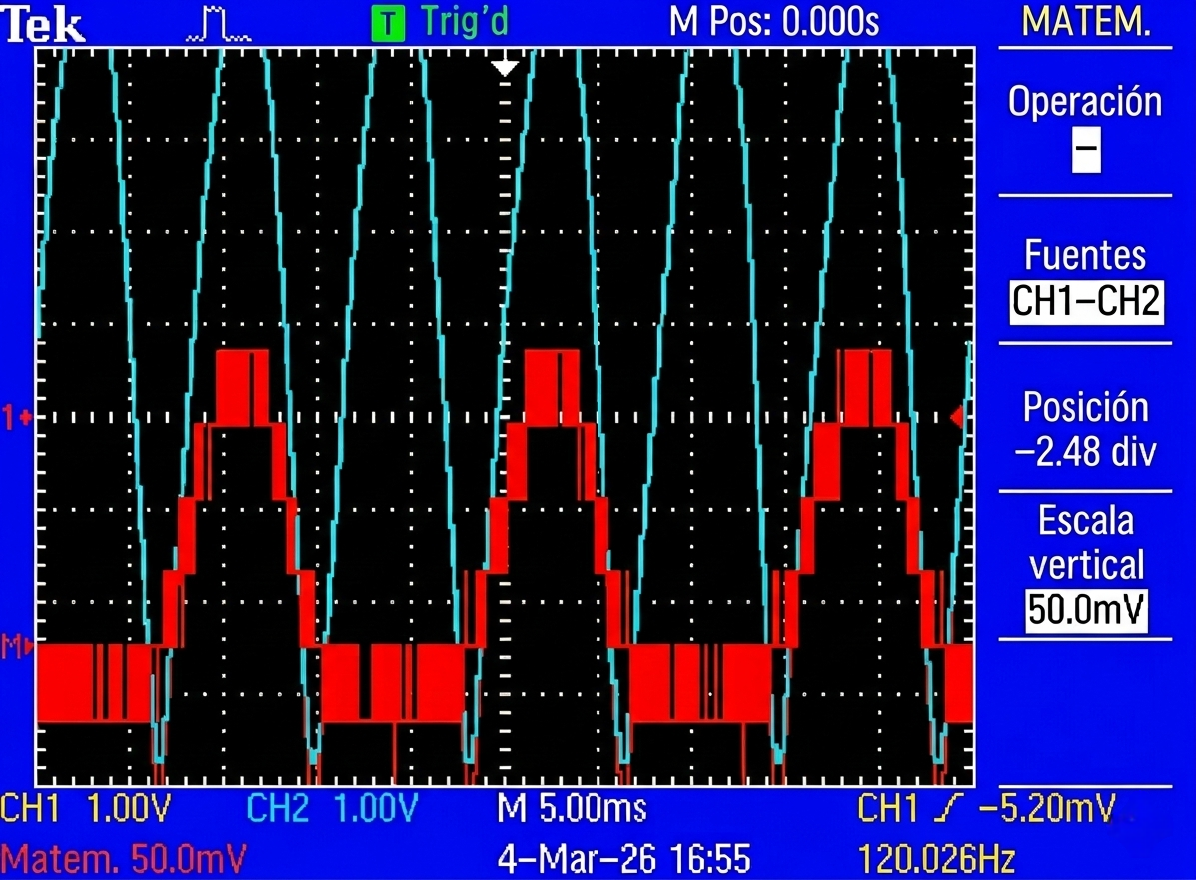
\includegraphics[width=0.45\textwidth]{IMAGENES/CorrienteDiodo.png} 
\caption{Forma de onda de la corriente en el diodo $D_1$.}
\label{fig:corrienteDiodo}
\end{center}
\end{figure}

El diodo entra en conducción únicamente durante el semiciclo positivo de la señal de alimentación (trazo azul), alcanzando una amplitud máxima ligeramente inferior a una división completa (aproximadamente 40 mV). Dado que la resistencia de prueba es de 
1 $\Omega$ , este valor se traduce directamente en una corriente pico de aproximadamente 40 mA, lo cual comprueba y valida el valor teórico calculado previamente de 39.2 mA.

\subsection{Análisis de comportamiento del circuito 2}

Haciendo un análisis rápido en el segundo circuito podemos darnos cuenta que el su comportamiento no es muy diferente al anterior, ya que ambos mantienen la misma configuracion con la unica diferencia de que este último tiene los diodos con la polaridad invertida,
lo cual nos indica que ahora el diodo $D_1$ conduce en el semiciclo negativo y el diodo $D_2$ en el positivo. Para comprobarlo, utilizamos el osciloscopio para ver el comportamineto del diodo $D_1$ de manera gráfica.

\begin{figure}[H]%[!ht]
\begin{center}
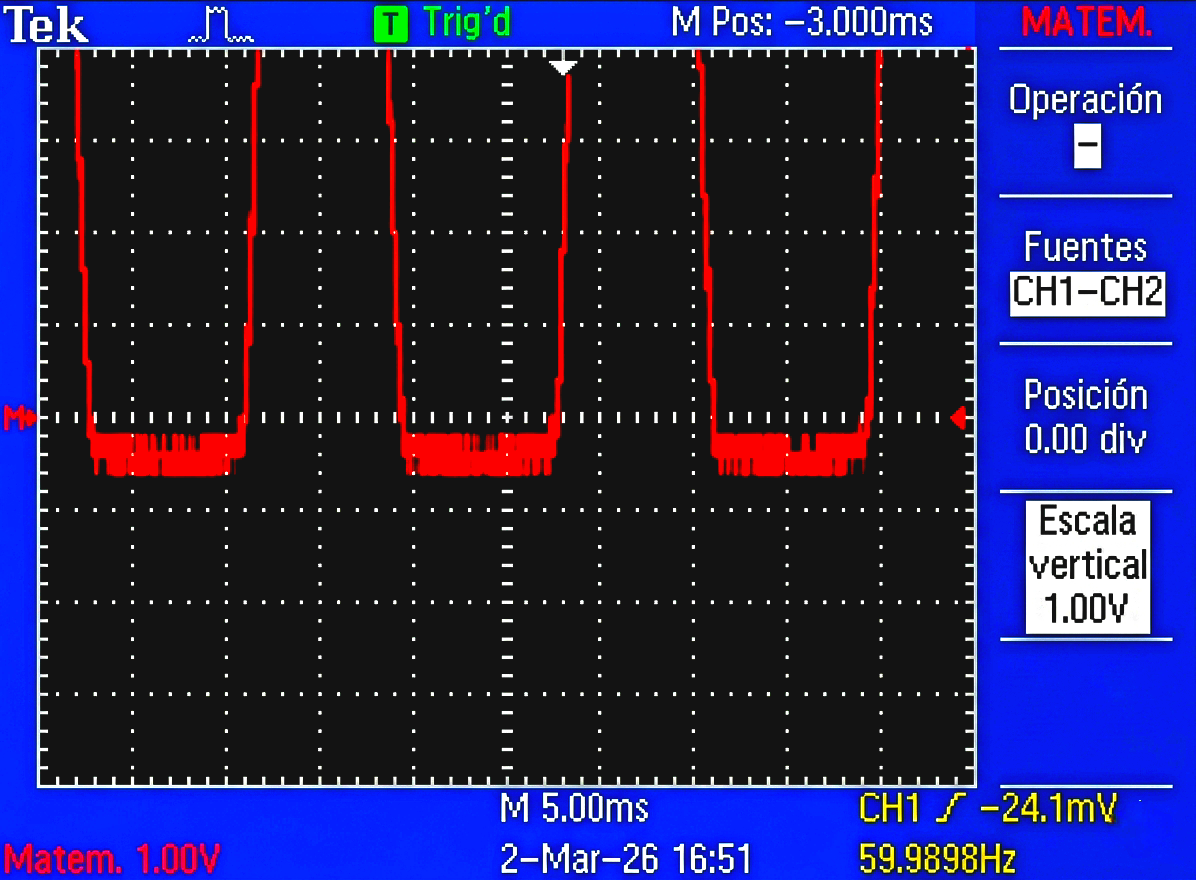
\includegraphics[width=0.45\textwidth]{IMAGENES/VoltajeInverso.png} 
\caption{Forma de onda de la corriente en el diodo $D_1$ en el circuito 2.}
\label{fig:corrienteDiodo2}
\end{center}
\end{figure}

Los valores teóricos esperados son exactamente los mismos. $V_{R1} = 8.64 \Omega $

\subsection{Análisis de comportamiento del circuito 3}

En esta sección se evalúa la topología de puente de Graetz (4 diodos). Esta configuración prescinde de la derivación central del transformador, utilizando el devanado secundario en su totalidad para alimentar la carga $R_1$.

Al utilizar los extremos del secundario, el voltaje eficaz de entrada al puente es de 13.21 $V_{rms}$, lo que equivale a un voltaje pico total de: 

\[
    V = 13.21 V_{rms} \cdot \sqrt{2} = 18.68 V
\]

En un puente de diodos, la corriente siempre atraviesa dos semiconductores simultáneamente en cada semiciclo (D1 y D2 en el positivo; D3 y D4 en el negativo) . Por tanto, la caída de tensión en los diodos es de 1.4 V (0.7 V+0.7 V).
El voltaje pico teórico en la resistencia de carga ($R_1 = 220 \Omega$) es:

\[
    V_{R1} = 18.68 V -1.4 V = 17.28 V
\]

Aplicando las ecuaciones matemáticas para una señal rectificada de onda completa, los valores teóricos esperados son:

\[
    V_{prom} = \frac{V_{R1}}{\pi} = \frac{17.28}{\pi} = 5.50 V
\]

\[
    V_{rms} = \frac{V_{R1}}{2\sqrt{2}} = \frac{17.28}{2\sqrt{2}} = 6.10 V
\]

Para las corrientes:

\[
    I_{prom} = \frac{V_{prom}}{220} = \frac{5.50}{220} = 0.025 V
\]

\[
    I_{rms} = \frac{V_{rms}}{220} = \frac{6.10}{220} = 0.027 V
\]

Al analizarlo en el osciloscopio obtenemos las siguientes imagenes.

\begin{figure}[H]%[!ht]
\begin{center}
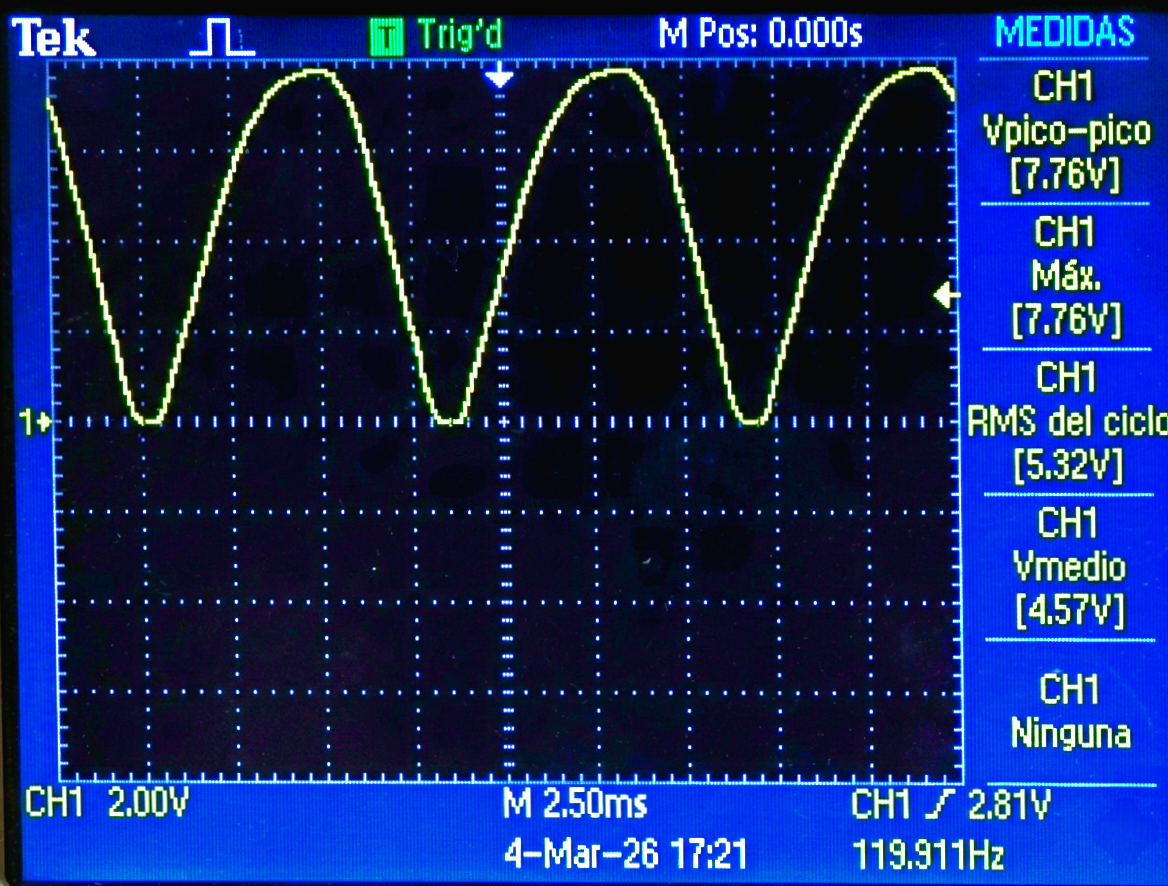
\includegraphics[width=0.45\textwidth]{IMAGENES/Voltaje.png} 
\caption{Voltaje en $R_1$ circuito 2}
\label{fig:VoltajeR1}
\end{center}
\end{figure}

Podemos observar la siguiente tabla que compara los resultados calculados y medidos con el osciloscopio y el multimetro

\begin{table}[H]
\centering
\begin{tabularx}{\columnwidth}{|c|X|X|X}
\hline
\textbf{Datos obtenidos} & \textbf{$V_prom$ (V)} & \textbf{$V_{rms}$ (V)} & \textbf{$V_{p}$ (V)}\\ \hline
Multímetro & 4.56 & 5.31  & 7.52\\ \hline
Cálculos & 5.50 & 6.10 & 8.64\\ \hline
Osciloscopio & 4.58 & 5.33 & 7.76\\ \hline
\end{tabularx}
\caption{Comparacion de voltajes calculados y medidos de $R_1$.}
\label{tablaComparativa2}
\end{table}

Durante el semiciclo en el que un par de diodos bloquea el paso de corriente (por ejemplo, $D_1$ apagado mientras $D_3$ y $D_4$ conducen), el voltaje inverso que debe soportar el diodo apagado se determina por mallas. 
En la configuración de puente, el diodo en inversa queda en paralelo con el devanado secundario y el diodo que está conduciendo en esa misma rama. Obtenemos:

\[
    V_{D1} = V + V_D = 18.68 V - 0.7 V = 17.98 V 
\]

En el osciloscopio se puede ver de la siguiente manera:

\begin{figure}[H]%[!ht]
\begin{center}
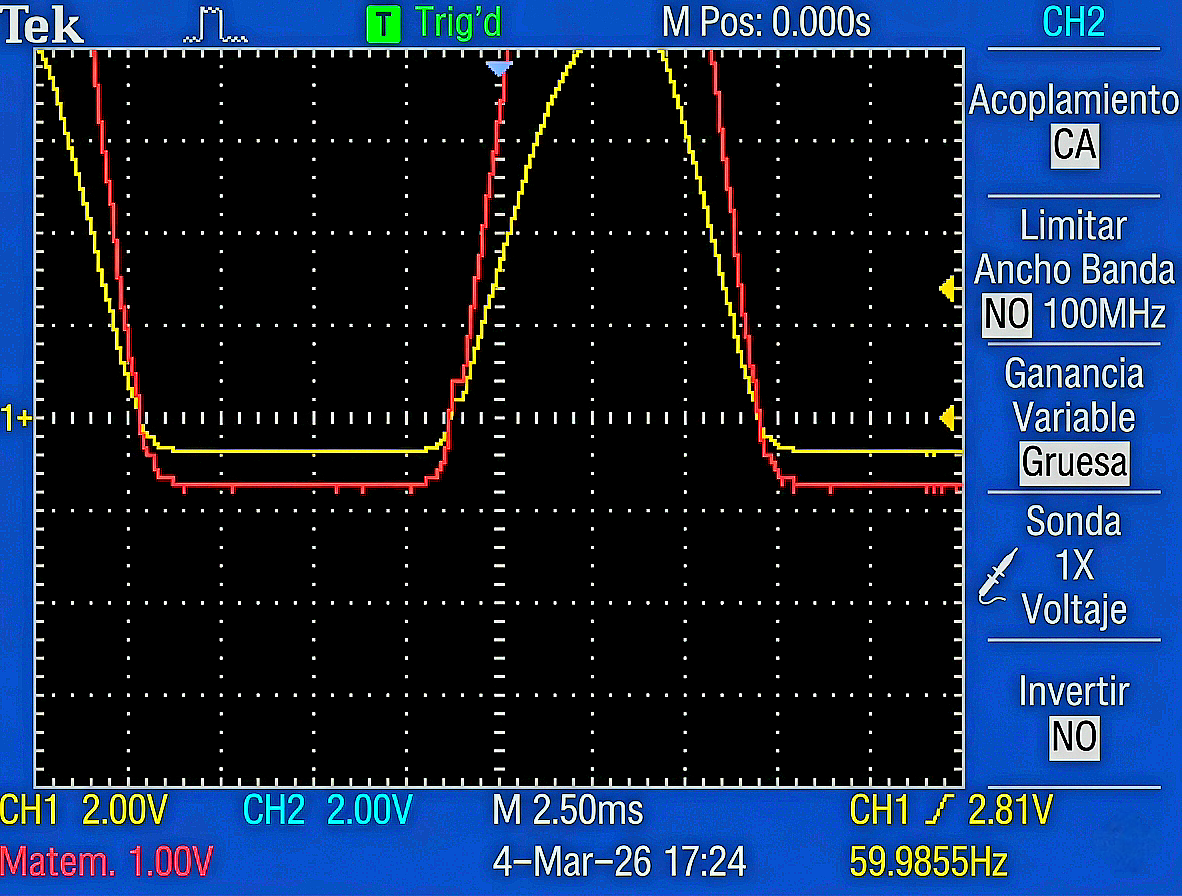
\includegraphics[width=0.45\textwidth]{IMAGENES/VoltajeD1_2.png} 
\caption{Voltaje en $R_1$ circuito 2}
\label{fig:VoltajeR1_2}
\end{center}
\end{figure}

\section{Simulación}

En esta sección se mostrará la simulación para el diodo IN4001 y 1N4148 para observar el comportamiento de voltaje y corriente en diodo al alterar la temperatura en ambos casos.

\begin{comment}
\begin{figure}[H]%[!ht]
\begin {center}

\includegraphics[width=0.45\textwidth]{IMAGENES/SIMULACION_4001.jpeg}
\caption{Simulación del diodo 1N4001 con variación de temperatura.}
\label{fig:sim_4001}
\end {center}
\end{figure}

\begin{figure}[H]%[!ht]
\begin {center}

\includegraphics[width=0.45\textwidth]{IMAGENES/SIMULACION_4148.jpeg}
\caption{Simulación del diodo 1N4148 con variación de temperatura.}
\label{fig:sim_4148}
\end {center}
\end{figure}
\end{comment}


\section*{a) Análisis de las regiones directa e inversa}

Analizar las variaciones de las regiones inversas y directas que existen en ambos 
diodos, y describir lo observado a medida que aumenta la temperatura.

En la región inversa de ambos diodos, a simple vista la corriente parece mantenerse como 
una línea recta constante en $0\,A$. Sin embargo, al ampliar la escala dentro de la simulación, 
se nota la presencia de pequeñas corrientes de fuga (la línea no es completamente plana). 

En el caso del 1N4148, a medida que aumenta la temperatura, la corriente inversa 
comienza a incrementarse incluso antes de llegar a los $0\,V$.

Por otro lado, en las regiones directas se puede apreciar cómo en el 1N4001 la corriente 
crece de manera estable. Además, es evidente que, a mayor temperatura, el diodo 
disminuye su barrera de potencial y no necesita tanto voltaje para empezar a conducir 
corriente.

\section*{b) Comparación del comportamiento térmico}

Comparar el comportamiento de ambos diodos y determinar cuál tiene un 
comportamiento más lineal con respecto a la temperatura.

Se puede observar en las gráficas cómo las curvas del 1N4001 se mantienen prácticamente 
paralelas entre sí en todos los casos de temperatura; es decir, mantiene un comportamiento 
lineal constante sin importar los incrementos térmicos. 

Por otro lado, el 1N4148 no se mantiene constante, sino que la pendiente de la curva cambia 
drásticamente entre cada variación de temperatura.

En conclusión, el diodo 1N4001 tiene un comportamiento más lineal y predecible con 
respecto a la temperatura en su región de conducción. Esto se debe a que es un diodo 
rectificador de potencia (diseñado para manejar mayores corrientes y disipar calor de forma 
estable), mientras que el 1N4148 es un diodo de pequeña señal y conmutación rápida, cuya 
unión es más pequeña y, por ende, más sensible a cambios térmicos drásticos.

\section*{d) Rangos de operación y aplicaciones}

\subsection*{Diodo Rectificador 1N4001}

\begin{itemize}
    \item \textbf{Rango de temperatura de operación (según hoja de datos):} $-55\,^{\circ}C$ a $+150\,^{\circ}C$ (temperatura de la unión).
    \item \textbf{Aplicaciones:} Uso general. Está diseñado para rectificar corriente alterna a 
    corriente directa a bajas frecuencias (como en fuentes de alimentación de 50/60 Hz), 
    protección contra polaridad inversa y en circuitos donde se manejan corrientes de 
    hasta $1\,A$ y voltajes de conmutación no muy rápidos.
\end{itemize}

\subsection*{Diodo de Señal 1N4148}

\begin{itemize}
    \item \textbf{Rango de temperatura de operación (según hoja de datos):} $-65\,^{\circ}C$ a $+150\,^{\circ}C$ 
    (en algunos empaques de vidrio soporta hasta $+200\,^{\circ}C$).
    \item \textbf{Aplicaciones:} Conmutación rápida (\textit{fast switching}). Se utiliza en procesamiento de 
    señales de alta frecuencia, circuitos lógicos digitales, multiplicadores de voltaje de 
    pequeña señal y en sistemas donde se requiere que el diodo cambie de estado (de 
    conducir a no conducir) en tiempos muy cortos (nanosegundos).
\end{itemize}

\section{Conclusiones}
\begin{itemize}
    \item \textbf{Flores Cornejo Gustavo Mauricio.}
    \newline En la presente práctica se pone en evidencia el comportamiento de 2 tipos de diodos de silicio, por lo que su comportamiento, como se puede ver en el desarrollo de la 
    práctica, es muy similar. Esta práctica sirve como base para comprender mucha de la parte teórica del diodo, como lo es su variación de parámetros al alterar la temperatura, además de visualizar el comportamiento de un diodo 
    real y comparalo con el comportamiento ideal. Como lo vimos en la sección del osciloscopio podemos observar una diagonal que representa el comportamiento del diodo cuando se encunetra polarizado inversamente, aquí retomamos el concepto 
    de la corriente de fuga que presenta el diodo. Mientras que el diodo ideal presenta una transición abrupta entre conducción y no conducción, el diodo real muestra una curva exponencial en la región directa y pequeñas corrientes en la región inversa. Como se observó en la sección del osciloscopio, la presencia de una línea diagonal en la región de polarización inversa retoma el concepto de la corriente de fuga, demostrando que el dispositivo no se comporta como un interruptor perfecto.

Finalmente, el análisis comparativo permitió entender que, aunque ambos diodos están fabricados en silicio, su diseño y aplicación influyen en su sensibilidad térmica y comportamiento eléctrico.
    
    \item \textbf{Muñoz Reyes Arturo Yabet.}
    \newline En conclusión, esta práctica comprobó de manera efectiva el comportamiento unidireccional y las características eléctricas de los diodos 1N4001 y 1N4148. Mediante mediciones se comprobó su funcionamiento en polarización directa e inversa, confirmando 
    que requieren un voltaje de activación típico de entre 0.6 V y 0.7 V para conducir la corriente. Finalmente, las simulaciones con variaciones de temperatura demostraron la sensibilidad térmica de estos componentes, destacando que el diodo  1N4001 mantiene una 
    mayor estabilidad frente al calor en comparación con el diodo 1N4148. Estos resultados subrayan la importancia de considerar tanto las especificaciones eléctricas como el comportamiento térmico al seleccionar semiconductores para aplicaciones en mecatrónica.

    \item \textbf{Morales Vásquez Miguel Ehecatl.} 
    \newline Tras la realización de esta práctica, se validó experimentalmente que el diodo semiconductor no presenta un comportamiento lineal, ya que requiere superar un voltaje de umbral (entre 0.5 y 0.7V para silicio) para permitir el flujo de corriente. 
    A través del contraste entre los modelos 1N4001 y 1N4148, se comprobó que mientras el primero es óptimo para rectificación de potencia por su capacidad de corriente, el segundo destaca en aplicaciones de alta frecuencia debido a su reducido tiempo de recuperación inversa. 
    Finalmente, el uso del osciloscopio en modo XY y la aplicación de la Ecuación de Shockley permitieron verificar cómo variables externas, especialmente la temperatura, alteran la barrera de potencial y la corriente de fuga, consolidando la comprensión de estos dispositivos en condiciones reales de operación

\end{itemize}



% if have a single appendix:
%\appendix[Proof of the Zonklar Equations]
% or
%\appendix  % for no appendix heading
% do not use \section anymore after \appendix, only \section*
% is possibly needed

% use appendices with more than one appendix
% then use \section to start each appendix
% you must declare a \section before using any
% \subsection or using \label (\appendices by itself
% starts a section numbered zero.)
%


\appendices
\section{Evidencias}

\begin{comment}
\begin{figure}[H]%[!ht]
\begin {center}

\includegraphics[width=0.45\textwidth]{IMAGENES/EVIDENCIA.jpeg}
\caption{Evidencia de evaluación de práctica.}
\label{fig:evidencia}
\end {center}
\end{figure}
\end{comment}



% references section

% can use a bibliography generated by BibTeX as a .bbl file
% BibTeX documentation can be easily obtained at:
% http://mirror.ctan.org/biblio/bibtex/contrib/doc/
% The IEEEtran BibTeX style support page is at:
% http://www.michaelshell.org/tex/ieeetran/bibtex/
%\bibliographystyle{IEEEtran}
% argument is your BibTeX string definitions and bibliography database(s)
%\bibliography{IEEEabrv,../bib/paper}
%
% <OR> manually copy in the resultant .bbl file
% set second argument of \begin to the number of references
% (used to reserve space for the reference number labels box)

%use following command to generate the list of cited references

\printbibliography

\begin{thebibliography}{00}
\bibitem{boylestad}
R. L. Boylestad and L. Nashelsky, \textit{Electronic Devices and Circuit Theory}, 10th ed. Upper Saddle River, NJ, USA: Prentice Hall, 2009.

\bibitem{1N4001}
onsemi, ``1N4001 -- 1.0 A Standard Recovery Rectifier,'' Datasheet, 2023. [Online]. Available: https://www.onsemi.com/pdf/datasheet/1n4001-d.pdf. [Accessed: Feb. 24, 2026].

\bibitem{1N4148}
onsemi, ``1N4148 -- Small Signal Switching Diode,'' Datasheet, 2023. [Online]. Available: https://www.onsemi.com/pdf/datasheet/1n4148-d.pdf. [Accessed: Feb. 24, 2026].
\end{thebibliography}

% that's all folks
\end{document}